\subsubsection{\stid{2.11} BOLT: Lightning Fast OpenMP}\label{subsubsect:bolt}

\paragraph{Overview}

OpenMP is central for several applications that target Exascale,
including ECP applications, to exploit on-node computational
resources.  Unfortunately, current production OpenMP runtimes, such as
those that ship with Intel and GNU compilers, are inadequate for the
massive and fine-grained concurrency expected at the Exascale level.
These runtimes rely on heavy-handed OS-level threading strategies that
incur significant overheads at fine-grained levels and exacerbate
interoperability issues between OpenMP and internode programming
systems, such as MPI and OpenSHMEM.  Our solution is a production
quality OpenMP runtime (called BOLT) that leverages user-level threads
instead of OS-level threads (e.g., Pthreads).  Due to their
lightweight nature, managing and scheduling user-level threads incurs
significantly less overheads.  Furthermore, interoperability between
BOLT and internode programming systems opens up new optimization
opportunities by promoting asynchrony and reducing hardware
synchronization (atomics and memory barriers).  Initial studies on
this proposal can be found in \cite{amer2018, ccgrid, ppopp}. This
report briefly summarizes the issues in OpenMP runtimes that rely on
OS-level threading, describes BOLT as the solution to this challenge,
the current status in the BOLT effort, and the next steps for further
improvements.

\paragraph{Key Challenges}

The growing hardware concurrency in High Performance Computing (HPC)
cluster nodes is pushing applications to chunk work more fine-grained
to expose parallelism opportunities.  This is often achieved through
nested parallelism either in the form of parallel regions or by
explicit tasks.  Nested parallel regions can potentially cause
oversubscription of OS-level threads to CPUs and thus lead to
expensive OS-level thread management.  Such heavy costs usually
outweigh the benefits of increased concurrency and thus compel the
OpenMP programmer to avoid nested parallel regions altogether.  Such
workaround, however, not only causes poor resource utilization from
insufficient parallelism but is also not always possible.  For
instance, the nested level could be outside the control of the user
because it belongs to an external library that also uses OpenMP
internally.  Internode programming systems, such as MPI and OpenSHMEM,
are not aware of OpenMP semantics, such as the notion of an OpenMP
task.  What these internode systems understand is the low-level
threading layer used by OpenMP, such as Pthreads.  This threading
layer serves as the interoperability medium between OpenMP and the
internode programming system and has a direct impact on performance.
It is notoriously known that OS-level thread safety in production MPI
libraries suffers significant performance issues. While continued
progress on improving OS-level thread safety in these important
internode programming systems is crucial for traditional
interoperability, we propose in this work exploring an orthogonal
direction that assumes a more lightweight interoperability layer.

\paragraph{Solution Strategy}

Both fine-grained parallelism and interoperability issues suffer from
the heavy nature of working at the level of OS threads.  Our solution
to both challenges leverages user-level threads.  Using user-level
threads as the underlying threading layer for the OpenMP runtime
offers a significantly better trade-off between high concurrency and
thread management overheads.  This allows users to generate
fine-grained concurrency and oversubscription without worrying about
the performance collapse that is observed in current OpenMP runtimes.
Our OpenMP runtime, BOLT, is derived from the LLVM OpenMP runtime and
leverages Argobots, a highly optimized lightweight threading library,
as its underlying threading layer.  OpenMP threads and tasks are
spawned as Argobots work units and nested parallel regions are managed
through an efficient work-stealing scheduler.  Furthermore, new
compiler hints and runtime optimizations have been developed to allow
reducing thread management overheads even further~\cite{iwasaki2018}.
Interoperability improvements have also been demonstrated by having
BOLT interoperate with an MPI library (MPICH) through the Argobots
threading layer rather than OS-level threads.  Results showed that
this approach allows better communication progress and outperforms the
traditional Pthreads-level interaction~\cite{seo2018}.

\paragraph{Recent Progress}

Our recent development of BOLT mainly focuses on efficient OpenMP
thread scheduling and management~\cite{BOLT}. BOLT takes substantial
advantage of its base implementation of LLVM OpenMP in terms of ABI
compatibility and coverage of functionalities, while we found the
necessity of further performance optimizations to fully exploit
fine-grained OpenMP parallel regions. After simple replacement of
Pthreads call sites with Argobots functions, we adopted several
resource management optimizations to reduce contentions and promote
reuse of resources. Thanks to low-level scheduling functions exposed
by Argobots, BOLT could implement OpenMP affinity tailored to a
ULT-based runtime. Our study also  the importance of a thread
coordination algorithm: it determines how to synchronize with other
threads (e.g., busy wait or suspension). To get the optimal
performance, existing runtime systems need to tune the wait policy
parameter based on the level of oversubscription, while our advanced
thread coordination algorithm in BOLT transparently keeps good
performance regardless of the degree of thread oversubscription. As
shown in Figure~\ref{fig:sollve-bolt}, BOLT achieves similar
performance compared with leading state-of-the-art OpenMP runtimes
under flat parallelism, while outperforming all the existing runtimes
under nested parallelism.

\begin{figure}[t]
  \centering
  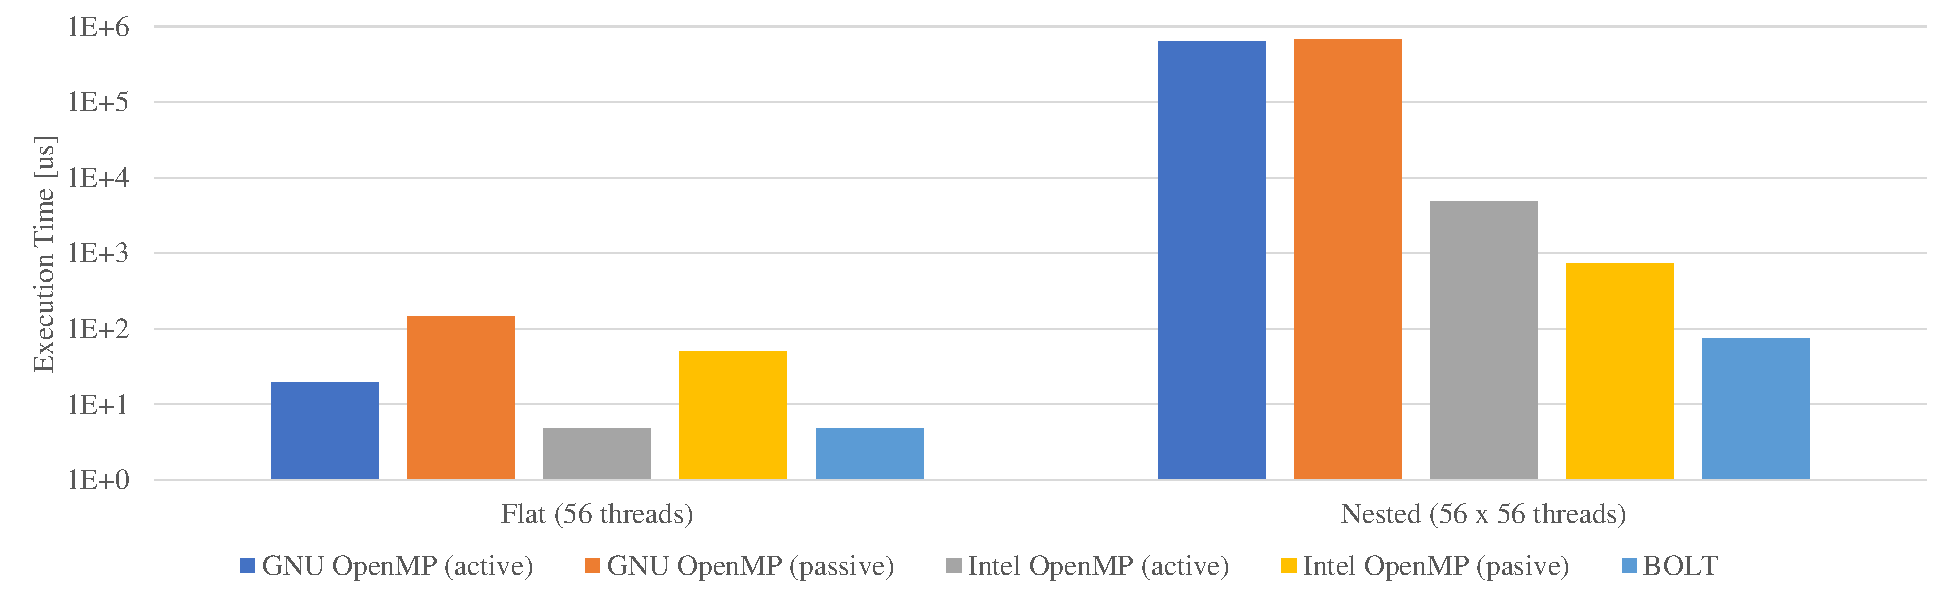
\includegraphics[width=0.9\columnwidth]{projects/2.3.2-Tools/2.3.2.11-SOLLVE/SOLLVE-BOLT.pdf}

  \caption{\label{fig:sollve-bolt}Performance of parallel regions on a
two-socket Intel Skylake machine (56 cores in total). GNU OpenMP 8.0
and Intel OpenMP 17.2.174 are used. The flat benchmark creates 56
OpenMP threads while the nested 56 OpenMP threads each of which opens
an inner parallel region with 56 threads. We changed the wait policy
for GNU and Intel OpenMP. See the paper \cite{BOLT} for details.}

\end{figure}

We note that design and implementation of BOLT are highly regarded in
the HPC community. The most significant achievement is the Best Paper
Award at PACT '19; our paper on BOLT, titled ``BOLT: Optimizing OpenMP
Parallel Regions with User-Level Threads''~\cite{BOLT} won a Best
Paper Award at the 28th international conference on Parallel
Architectures and Compilation Techniques (PACT '19), which is
considered to be a top tier venue in this field.

The latest BOLT 1.0rc2 has been upgraded to be compatible with LLVM
OpenMP 9.0, which further improves performance and functionalities
especially for GPU offloading. We also created a development branch
that keeps reflecting the latest changes in the LLVM OpenMP's master
branch so that BOLT users can try the up-to-date features with ULT
support. Interaction and integration are a critical piece for the BOLT
project. Our effort in the SOLLVE Spack package, which was one of the
SOLLVE milestones, aims at a tighter integration with the other
components of the SOLLVE project. Our efforts include interaction and
evaluation with (1) ECP applications that have fine-grained
parallelism such as nested parallel regions and tasking (e.g., ECP
SLATE) and (2) runtime systems via the Argobots layer (for example,
MPICH and Open MPI) that can take advantage of ULT's lightweight
synchronization for resource management.

\paragraph{Next Steps}

One of the largest advantages of BOLT is an underlying lightweight
thread implementation, flexible scheduling, and high interoperability
thanks to Argobots. The following list includes our next plans:

\begin{enumerate}

\item Investigates opportunities of utilizing lightweight threads for
other optimizations in the context of OpenMP. BOLT successfully
enhanced performance of OpenMP threads, while it remains unexplored
how BOLT could elevate performance of other parallel units (e.g.,
data-dependent tasking and GPU offloading). We are planning to
investigate room for optimizations and implement them with
evaluation.

\item Improves the interoperability with MPI runtimes. Although the
basic scheme is provided via the Argobots layer, its optimization is
premature. In addition to improvement of the interoperability between
MPI and Argobots, we will investigate an OpenMP-specific
interoperability issue if exists.

\item Collaborates with more applications and users. BOLT has gained
the attention of the HPC community, but its reach and impact remain
limited. In order to find potential room for optimizations and
evaluate the performance of BOLT in real workloads, we further
investigate other applications, including ECP ones, that BOLT can
benefit.

\end{enumerate}
